\documentclass[review, onefignum, onetabnum]{siamart171218}
% This is information that is shared between the main document and any
% supplement. If no supplement is required, then this information can
% be included directly in the main document.


% Packages and macros go here
\usepackage{lipsum}
\usepackage{amsfonts}
\usepackage{graphicx}
\usepackage{epstopdf}
\usepackage{algorithmic}
\usepackage{tikz}
\usepackage{subcaption} 
\usepackage{pc_math}
\usepackage{amssymb}
\usepackage{bbm}
% \usepackage[color=gray!60]{todonotes}
\usepackage[disable, color=gray!60]{todonotes}
% \usepackage{caption}
% \usepackage{hyperref}
\graphicspath{{fig/}}

\tikzstyle{major}=[circle, fill=blue!50, minimum size=10pt, line width=0mm, inner sep=0pt, draw=black]
\tikzstyle{minor} = [major, fill=orange!80, draw=black]
\tikzstyle{focus} = [minor, line width=.2mm, inner sep=1pt, draw=black]
\tikzstyle{edge} = [draw,line width=.3mm, -, gray!120]
\tikzstyle{gone} = [edge,  densely dotted]
\tikzstyle{arrow} = [draw,line width=.2mm, ->, gray!120]


\tikzstyle{weight} = [font=\small]

\ifpdf
  \DeclareGraphicsExtensions{.eps,.pdf,.png,.jpg}
\else
  \DeclareGraphicsExtensions{.eps}
\fi

% Add a serial/Oxford comma by default.
\newcommand{\creflastconjunction}{, and~}

% Used for creating new theorem and remark environments
\newsiamremark{remark}{Remark}
\newsiamremark{hypothesis}{Hypothesis}
\crefname{hypothesis}{Hypothesis}{Hypotheses}
\newsiamthm{claim}{Claim}

% Sets running headers as well as PDF title and authors
\headers{Adaptive Voter Models}{P. Chodrow, P. J. Mucha}

% Title. If the supplement option is on, then "Supplementary Material"
% is automatically inserted before the title.
\title{Symmetry-Breaking in Adaptive Voter Models\thanks{Submitted to the editors \today.
\funding{This work was funded by the NSF (1122374).}}}

% Authors: full names plus addresses.
\author{Philip S. Chodrow\thanks{Operations Research Center, Massachusetts Institute of Technology, Cambridge, MA, 02139 and Laboratory for Information and Decision Systems, Massachusetts Institute of Technology, Cambridge, MA, 02139
  (\email{pchodrow@mit.edu}, \url{http://www.philchodrow.github.io}).}
\and Peter J. Mucha\thanks{Carolina Center for Interdisciplinary Applied Mathematics, Department of Mathematics, University of North Carolina, Chapel Hill, NC 27599-3250, and Department of Applied Physical Sciences, University of North Carolina, Chapel Hill, NC 27599-3050. 
  (\url{http://mucha.web.unc.edu/}).}}

\usepackage{amsopn}
%%% Local Variables: 
%%% mode:latex
%%% TeX-master: "ex_article"
%%% End: 


\usepackage{color}
\usepackage{xcolor}
\colorlet{comment_purple}{blue!50!red}

\usepackage{todonotes}

\newcommand{\pjm}[1]{{\color{blue}[PJM: #1]}}
\newcommand{\pc}[1]{{\color{comment_purple}[PC: #1]}}
\ifpdf
  \hypersetup{
    pdftitle={Adaptive Voter Models},
    pdfauthor={P. Chodrow, P. J. Mucha}
  }
\fi
\externaldocument{supplementary}

\begin{document}
\maketitle

\begin{abstract}
	``Co-evolving" or ``adaptive" voter models (AVMs) are \pjm{Add something else here too?}\pc{What do you have in mind here?} natural systems for modeling the emergence of mesoscopic structure from local processes driven by conflict and homophily. 
	Because of this, many methods for studying the long-run behavior of AVMs have been proposed over the last decade. 
	However, most such methods are either restricted in scope, expensive in computation, or inaccurate in predicting important statistics.  
	In this work, we develop a novel, 2nd-order moment closure approximation method for studying the equilibrium mesoscopic structure of AVMs and apply it to binary-state rewire-to-random and rewire-to-same model variants with random state-switching. 
	This framework exploits an asymmetry in voting events that enables us to derive analytic approximations for the fast-timescale dynamics. 
	The resulting numerical approximations enable the computation of key properties of the model behavior, such as the location of the fragmentation transition and the equilibrium active edge density, across the entire range of state densities. 
	Numerically, they are nearly exact for the rewire-to-random model, and competitive with other current approaches for the rewire-to-same model. 
	We conclude with suggestions for both model refinement and extensions to more complex models. 
	
\end{abstract}

\begin{keywords}
	Networks, nonlinear dynamics, phase transitions, community structure
\end{keywords}
\begin{AMS}
	82B26, % Phase transitions (general)
	91D30, % Social networks
	91-08, % Computational methods in Game Theory, Economics, Social and Behavioral Sciences
	91B14  % Social Choice
\end{AMS}

\section{Introduction} \label{sec:intro}

	A common feature of social networks is assortativity, the tendency of people who share similar attributes to interact more intensely or frequently than those who do not.
	Assortativity can be beneficial, allowing communities of individuals who share common beliefs or experiences to pursue shared goals. 
	On the other hand, assortativity can also restrict flows of information and resources between homogeneous groups. 
	Recent scrutiny, for example, has fallen on the role of online platforms in promoting political polarization by allowing users to micromanage their contacts and information sources \cite{Bakshy2015,Anagnostopoulos2014}. 
	Polarization in turn contributes to undesirable social and political outcomes, including the propagation of untruthful reporting\cite{Lazer2018}, uncompetitive elections \cite{Abramowitz2006}, legislative deadlock \cite{Layman2006}. 
	It is therefore of importance to develop quantitative theories of how opinion-based sorting drives large-scale network assortativity. 

	Assortativity in networks has often been studied within the framework of \emph{community structure}, a study that extends at least as far back as the reporting of the now-infamous Zachary Karate Club network \cite{Zachary1977} in which polarized factions of martial artists zfissioned into separate clubs.  
	Informally, a network displays community structure when it can be partitioned into groups in such a way nodes within each group are strongly connected within their group and only weakly connected beyond their group. 
	The model-based approach to the study of communities is largely statistical, dominated by the stochastic blockmodel and its variants.  
	The stochastic blockmodel is a planted-partition model that assigns a probability to each possible configuration of community labels. 
	Communities community-detection in this context is treated as a statistical inference problem, an approach which has the benefit of  mathematical grounding and useful theoretical connections to the popular practical method of modularity maximization \cite{Newman2016a}. 
	Sophisticated methods have recently emerged that incorporate additional graph metadata \cite{Peel2016,Newman2016b} or Bayesian model selection \cite{Peixoto2017a,Peixoto2017d}. 
	See \cite{Shai2017} for a useful review of recent developments and discussion of illustrative case studies. 
	\todo{Peter, this might be a good place to add references, including to some of your own favorite papers.}

	While community-structured networks appear to be ubiquitous, relatively few quantitative stories exist to describe how they come to display or maintain that structure. 
	A model due to \cite{Kumpula2007} mechanistically generates communities using two purely topological mechanisms: triadic closure and global attachment. 
	This model produces attractive, tunable community structures, but its purely topological structure makes it inappropriate for studying the interaction between topology and agent attributes. 
	Inspired by the classical Schelling model of urban segregation \cite{Schelling1979}, the authors of \cite{Henry2011} consider a network in which agents are assigned an immutable attribute vector that may model demographics or opinions. 
	Agents are allowed to rewire their connections to dissimilar partners, selecting new ones via global attachment, with the aversion to dissimilarity governed by a parameter. 
	As the authors prove, the model always generates segregated communities for any nonzero degree of dissimilarity aversion. 
	However, the node attributes are generated exogenously to the system dynamics.
	This model is therefore appropriate for studying assortativity based on immutable traits such as skin color, but less appropriate for opinions, over which the views of associates may have considerable influence.
	Because the node attributes are exogeneous to the system dynamics, this model is most appropriate for studying demographic segregation, rather than mutable opinions. 
	At the other extreme is the classical voter model \cite{Clifford1973,Holley1975}, in which node attributes change in response to local influence but the network topology remains constant.

\pjm{The previous paragraphs are really heavy on community structure. We want to streamline this to get the focus more on coevolving/adaptive systems.}
	Over the last decade, a class of coevolutionary models has emerged that enforces dynamical coupling between node attributes and edge topology, and which are therefore well suited to the study of opinion-based assortativity.
	This class, which we will refer to collectively as \emph{adaptive voter models} (AVMs), are endowed with two dynamical update steps. 
	In a \emph{voting} step, a node adopts the opinion of one of its neighbors according to a specified update rule. (We refer to this opinion-adoption as ``voting'' to distinguish from other opinion changes considered later in the paper.)
	In a \emph{rewiring} step, a node cuts its ties to a disagreeing neighbor and selects a new neighbor from the remainder of the social graph. 
	The relative frequency of rewiring and voting events is governed by a tuneable parameter. 
	These dynamics combine to generate polarized networks of opinion-based communities. 
	AVMs therefore offer a fully endogenous model of fragmentation, polarization, and segregation in information networks. 
	Beyond their social relevance, AVMs are interesting as theoretical objects, displaying phase transitions, metastability, and other rich behavior. 
	However, the nonlinearity driving this rich behavior renders AVMs extremely difficult to analyze even approximately. 
	Existing methods are typically significantly restricted at least one of scope, computational complexity, or accuracy, and often fail to provide significant physical intuition driving observed behaviors. 
	It is therefore of interest to seek new approximation schemes for this class of models. 
	Our aim in this paper is to use a seemingly under-noted observation to develop a class of approximation methods that both explain qualitative behaviors in these systems and provide unprecedented combinations of scope, computational efficiency, and accuracy. 

	The paper is structured as follows. 
	We first review AVMs in \Cref{sec:AVMs}, defining their update dynamics, discussing the behavior of their most interesting observables, and surveying previous approaches for studying them. 
	In \Cref{sec:AVM_noisy}, we describe the version of the AVM that is the focus of our present study, which modifies the models of \cite{Durrett2012} by introducing a small rate of random opinion-switching. 
	As a benefit of this additional randomness, the resulting dynamics provide for the existence of a well-defined equilibrium measure governing the long-term system behavior. 
	The existence of this measure contrasts with the trivial, fully-fragmented absorbing states of models without opinion switching, which is both realistic and analytically convenient. 
	Using this measure, we observe an asymmetry in the structure of voting events, motivating it theoretically and then demonstrating it in simulation data. \pc{Add this fig back in} 
	We leverage this asymmetry in \Cref{sec:analytic} to construct a highly accurate approximation scheme for the subcritical behavior of the AVM. 
	Our approximation also generates useful intuition concerning a previously mysterious qualitative difference between the phase transitions of two variants of this adaptive system.
	We next use simple mean-field arguments to extend the approximation past the phase transition, thereby enabling us to estimate the quasistable manifold--the arch--along which the equilibrium distribution of the opinion counts and edge densities concentrates.
	We again demonstrate favorable scope, accuracy, and computational complexity in comparison to existing methods.
	We close in \Cref{sec:discussion} with a discussion of promising extensions, both to our approximation methodology and to the model itself. 
	
\section{Adaptive Voter Models} \label{sec:AVMs}
	
	Adaptive Voter Models (AVM) form a class of first-order, discrete-time Markov processes on a space of states of the form $G = (\mathcal{N}, \mathcal{L}, \mathcal{E})$, where $\mathcal{N}$ is the set of nodes and $\mathcal{E}$ is the set of edges; $(u,v) \in \mathcal{E}$ means that an edge linking nodes $u$and $v$ is present in $\mathcal{G}$.
	\footnote{Adaptive network dynamics have also been studied in the context of epidemic spreading \cite{Marceau2010,Lee2017} and game theory \cite{Malik2016}; however, we will not consider these models here.} \pjm{We should find some other references to add to this footnote, and perhaps also move this footnote into a sentence in the Introduction} 
    The vector $\mathcal{L}$  node labels maps $\mathcal{N} \rightarrow \mathcal{X}$ where $\mathcal{X}$ is an alphabet of possible label values. 
	The node set $\mathcal{N}$ is fixed, while both $\mathcal{L}$ and $\mathcal{E}$ evolve stochastically.
	The case $\mathcal{X} = \{0,1\}$, corresponding to binary-state dynamics, is most frequently considered. 
	Additional interesting features arise in multi-opinion dynamics \cite{Holme2006, Shi2013}; however, we will restrict to the binary-state case in this paper. 
	
	The time-evolution of an AVM is characterized by superimposed voting dynamics on $\mathcal{L}$ and edge-rewiring dynamics on $\mathcal{E}$. 
	Our model adds a third process in the form of random opinion switching, a mechanism first considered in \cite{Ji2013}. 
	The (discrete-time) stochastic dynamics $(\mathcal{E}(t), \mathcal{L}(t)) \mapsto (\mathcal{E}(t+1), \mathcal{L}(t+1))$ are specified as follows:
		\begin{enumerate}
			\item With probability $\lambda \in [0,1]$, \textbf{mutate}: uniformly sample a node $u\in \mathcal{N}$ and send sample $\mathcal{L}_u(t+1)  \sim \mathrm{uniform}(\mathcal{X}\setminus \{\mathcal{L}_u(t)\})$.  
			\item Otherwise (With probability $1-\lambda$),  sample an edge $(u,v) \in \mathcal{E}(t)$ uniformly from the set $\{(u,v):\mathcal{L}_u(t) \neq \mathcal{L}_v(t)\}$ of \emph{active} edges. Then, 
			\begin{enumerate}
				\item With probability $\alpha \in [0,1]$, \textbf{rewire}: delete the (undirected) edge $(u,v)$ and add edge $(u,w)$ selected according to one of the following two rules depending on the model variant being used. 
				In the \emph{rewire-to-random} model variant, $w$ is chosen uniformly from $\mathcal{N}\setminus \{u\}$. 
				In the \emph{rewire-to-same} variant, $w$ is chosen uniformly from the set $S_u = \{w' \in \mathcal{N}\setminus \{w\} | \mathcal{L}_{w'}(t) = \mathcal{L}_u(t)\}$. 
				\item Otherwise (with probability $1-\alpha$) \textbf{vote}:  $\mathcal{L}_u(t+1) \gets \mathcal{L}_v(t)$. 
			\end{enumerate}
		\end{enumerate}
	Incorporating random opinion-switching is attractive from a modeling perspective -- this process may be viewed as reflecting exogeneous influence, such as media sources, noisy communication, or idiosyncratic growth that may coexist with the minimal AVM dynamics.  
	Opinion-switching also has an important technical implication -- it is direct to show that, when $\lambda > 0$, the AVM is an ergodic Markov chain. 
	As a result, the model acquires an equilibrium measure supported on its state-space that governs its long term behavior. 
	
	\subsection{Phenomenology of AVMs}
		AVMs display rich behavior most typically studied through a standard set of summary statistics.  
		Let $n = \abs{\mathcal{N}}$ be the number of nodes, $m = \abs{\mathcal{E}(t)}$ the number of edges, and $c = {2m}/{n}$ the mean degree.
		Since the dynamics conserve $n$ and $m$, $c$ is time-independent and may be regarded as an additional system parameter. 
		Let $N_i(t) = \abs{\{u \in \mathcal{N} \;|\;\mathcal{L}_u(t) = i \}}$ be the number of nodes holding opinion $i$ at time $t$. 
		We define $\q(t) = n^{-1}\left(N_0(t), N_1(t)\right)$ to be the vector of opinion densities.
		Let $M_{ij}(t) = \abs{\{(u,v) \in \mathcal{E} \;|\; \mathcal{L}_u(t) = i,\; \mathcal{L}_v(t) = j \}}$ be the number of \emph{oriented} edges between nodes of opinion $i$ and nodes of opinion $j$. 
		Note that $M_{ij}(t) = M_{ji}(t)$ and $\sum_{i,j \in \mathcal{X}} M_{ij}(t) = 2m$ at all times $t$.
		We call an edge $(u,v)$ ``active'' if it is discordant, that is, $\mathcal{L}_u(t) \neq \mathcal{L}_v(t)$. 
		Let $\X(t) = m^{-1}\left(M_{00}, M_{01}, M_{10}, M_{11}\right)$ be the vector of edge densities. 
		We define the scalar $\rho(t) = M_{01} + M_{10}$ to be the overall density of active edges. 
		For notational compactness, we will repress the argument $t$ when no possibility of confusion arises.
		
		When $\lambda = 0$, any fully-fragmented state with $\rho = 0$ is absorbing. 
		Such a state consists of one or more connected components within each of which the labels are internally identical. 
		As noted in both \cite{Holme2006} and \cite{Durrett2012}, there is an intriguing phase transition in the final value of $\q$, the details of which depend on the precise model variant. 
		In each variant, there is a critical value of $\alpha$, depending on $\q(0)$, such that, if $\alpha \geq \alpha^*(\q(0))$, $\q \approx \q(0)$. 
		On the other hand, if $\alpha < \alpha^*(\q(0))$, the final value of $\q$ is governed by a bimodal distribution whose modes are independent of $\q(0)$, determined instead by $\alpha$, $c$, and the rewiring mode. \pjm{Double-checking your intent here, it's only bimodal for two opinions, right? Can we simply drop the word ``bimodal'' here and everything is then okay?}\pc{Strictly speaking yes, but I think it's clearer to be concrete about the behavior in the binary-state case to which we have restricted. I've added a reminder to the paragraph before that we are in binary world. Think that's enough?}
		In the rewire-to-same case, the modes lie at $\q = (1,0)$ and $\q = (0,1)$, while in the rewire-to-random case, both components of the modes are nonzero and depend on $\alpha$ and the mean degree $c$. 
		This phase transition marks the point at which the rewiring dynamics outstrip the voting process, and therefore also corresponds to a transition in the time to reach the final state \cite{Holme2006,Rogers2013}. 
		In \cite{Durrett2012}, the authors show that the phase transition also corresponds to the properties of a \emph{quasistable manifold} that is well approximated as a concave parabola in the $\q_1$-$\rho$ plane which the authors accordingly dub ``the arch.'' 
		The arch expresses $\rho^*$, the expected discordant edge density, as a function of $\alpha$ and $\q$. 
		\begin{figure}
		 	\centering
		 	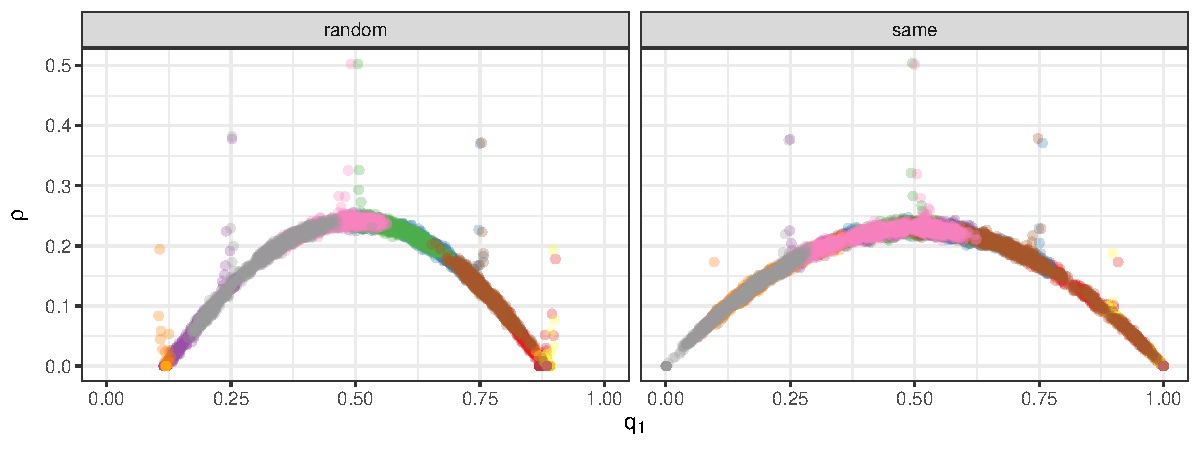
\includegraphics[width=.7\textwidth]{arch_illustration}
		 	\caption{Quasi-stable arches in $\q-\rho$ space. 
		 	Points give traces of 10 sample simulations of AVMs with $n = 10^4$ and $c = 4$, run for $\times 10^7$ steps and sampled at intervals of $5\times 10^3$. 
		 	The horizontal axis gives the density $q_1$ of opinion-$1$ nodes, and the $y$-axis the active edge density $\rho$. 
		 	The rewiring rate $\alpha$ is $0.5$ for the rewire-to-random arch and $0.3$ for the rewire-to-same arch.} 
		 	\label{fig:arch_illustration}
		\end{figure} 
		A typical evolution of an AVM will converge rapidly toward a point on the arch, and then diffuse slowly along it toward one of the two points at the base, as shown in \Cref{fig:arch_illustration}.
		As remarked in \cite{Durrett2012} and illustrated by our simulation results plotted in  \Cref{fig:arch_illustration}, the rewire-to-random arch is supported on a proper subinterval of $[0,1]$ whenever $\alpha >0$, while the rewire-to-same arch is supported on the entirety of $[0,1]$. 
		
		This difference in the supports of the arches for the two model variants is counterintuitive. 
		In particular, when one of the opinion populations is small, the active edge density $\rho$ in the rewire-to-same model is actually \emph{higher} than in the rewire-to-random model with the same opinion counts and parameters.  
		This is in marked contrast to the expectation that the rapid sorting of edges via rewire-to-same would presumably lead to  smaller active edge densities. \pjm{Is it worth making a comment about how the pair approximation algebra works? That is, we have an ``explanation'' (poor perhaps) at that level, but I don't think we ``understand'' it.}\pc{Inclined to pass here, but I have added language below noting that PA and AMEs get some qualitative aspects right. Do you think that does enough work?}
		While some approximation schemes \cite{Durrett2012} replicate this qualitative difference, to our knowledge no physical or mathematical insight into this phenomenon is available. 

		When $\lambda > 0$, the ergodicity of the Markov chain implies that no state is absorbing. 
		Instead, a typical sample from the equilibrium distribution of $\mathcal{G}$ display bifurcated community structure, with dense connections within opinion groups and sparser connections between groups. 
		\Cref{fig:sample} shows a single realization for a small AVM. 
		We note that this realization replicates the visual properties of other networks that have a large-scale organization into two communities. 
		This behavior of the mutating AVM thus makes it a more realistic model of social processes with persistent disagreement. 
		It also enables us to study properties of the non-mutating AVM -- when we allow $\lambda$ to grow small, the equilibrium measure concentrates around the arch observed in the $\lambda = 0$ case. 
		\begin{figure}
			\centering
			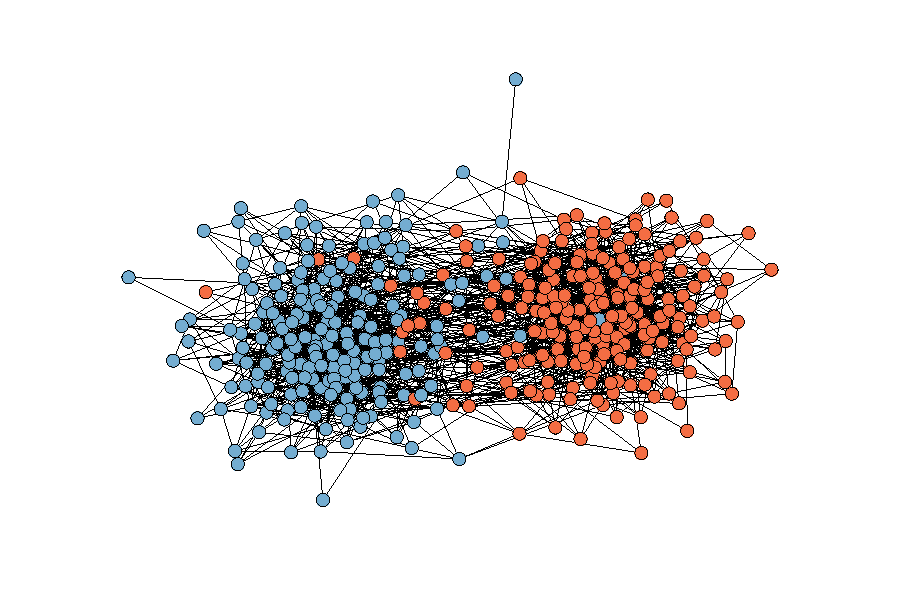
\includegraphics[width=.7\textwidth]{network_sample}
			\caption{Sample from the equilibrium distribution of a rewire-to-random AVM with $n = 400$ agents, mean degree $c = 10$, rewiring rate $\alpha = 0.9$, and mutation rate $\lambda = 0.01$. The active edge density is $\rho = 0.12$.} \label{fig:sample}
		\end{figure}
		The central analytical task is therefore to estimate the behavior of $\rho$ as a function of the parameters $\lambda$, $\alpha$, and $c$, as well as the opinion density $\q$.
		\footnote{Recent papers have noted other additional phenomena of interest, such as approximate conservation laws \cite{Toruniewska2017} and structural behavior near the phase transition $\alpha^*$ \cite{Horstmeyer2018}; however, we will not pursue these themes further here.}
		Many previous studies have focused on subsets of this task.
		The most restricted task is to estimate the phase transition $\alpha^*$ in the case of symmetric opinion densities  $\q = \left(\frac{1}{2}, \frac{1}{2}\right)$.
		A common baseline for comparison in this literature is the all-purpose pair approximation (PA), which can be conveniently computed in closed-form. 
		However, the PA is highly inaccurate with respect to both the location of the phase transition $\alpha^*$ and active edge density $\rho$ \cite{Demirel2012, Durrett2012}. 
		More specialized methods are required to obtain quantitatively reasonable estimates. 
		In \cite{Basu2015a}, the authors apply stopping-time arguments to give the first rigorous proof of the existence of a phase transition known to us. 
		However, their results apply only to dense graphs and do not explicitly construct the value of $\alpha^*$ or even show the existence of a single, well-defined phase transition. 
		In \cite{Bohme2011}, a master equation-type approach is used to construct accurate estimates of the phase transition for the rewire-to-same model with symmetric opinion densities. 
		Computation requires a bisection search in $\alpha$ for which each function evaluation corresponds to finding the largest eigenvalue of a $(c-1) \times (c-1)$ matrix. \pjm{Actually, shouldn't $c$ be $k_\mathrm{max}$ here?}\pc{You would expect that, but they employ a regularity assumption that allows them to work with the smaller matrix, so it is indeed $c-1$.}
		
		Other authors attempt to derive not only the phase transition $\alpha^*$ but also the supercritical active edge density $\rho$ in the symmetric opinion case. 
		For example, the authors of \cite{Demirel2012} uses an approximate master equation approach, with reasonable quantitative results for the rewire-to-same case. 
		In \cite{Silk2014}, the authors convert an approximate master equation system into a single PDE, which they solve analytically. 
		Despite the elegance of the approach, the agreement with simulations is not strong. 
		The authors of \cite{Ji2013}  develop a novel analytical framework for studying the quasistable active edge density, and even incorporate random opinion-switching, but their scheme contains constant terms that must be estimated from data. 
			
		To our knowledge, the only attempt to the complete arch for $\q \neq \left(\frac{1}{2}, \frac{1}{2}\right)$ is given in \cite{Durrett2012}, which applies pair approximations as well as large systems of approximate master equations (AME, \cite{Gleeson2013}) to rewire-to-random and rewire-to-same model variants. 
		The AME estimates for the arches significantly improve on the pair approximation, and display some of the qualitative features observed in simulations. 
		The results obtained by AME, however, possess several limitations. 
		They are intuitively opaque, making it difficult to understand why their predictions should deviate from simulations in the ways observed.  
		Furthermore, they are relatively computationally intensive (compared to, say, mean-field or pair-approximation approaches); in particular, the AME results in \cite{Durrett2012} requires the numerical solution of $\Theta(k_\mathrm{max}^2)$, where $k_\mathrm{max}$ is the largest node-degree expected to emerge in the course of a simulation, and therefore depends on the mean degree $c$. 
		This scheme quickly becomes impractical even for modest $c$. 

	\section{Analytical Methods}
	    We now develop an analytical approximation framework for estimation of the arch. 
	    The strategy is to conduct a perturbative analysis about the fully fragmented state $\rho = 0$. 
	    When $\lambda = 0$, the fragmented state is trivially stable and no useful analysis is possible. 
	    In contrast, when $\lambda > 0$, the system is subject to small fluctuations induced by the random-opinion switching, which may potentially drive the system to a qualitatively new region of phase space. 
	    We now explore this perturbative approach in detail. 
	    
	    Consider the genesis via opinion-switching of a single dissenting node $u$. 
	    Because $\mathcal{G}$ is otherwise uniform on its connected components, the fast-timescale dynamics concentrate in the neighborhood of $u$. 
    	We can distinguish two qualitative regimes: 
    	\begin{enumerate}
    		\item \textbf{Subcriticality:} With high probability, the dissenting opinion on $u$ is eventually either snuffed out by $1\mapsto 0$ voting or quarantined by rewiring. 
    		Subsequent opinion-switches will generate similar ``outbreaks,'' which are then similarly contained.   
    		\item \textbf{Supercriticality:} With nonzero probability, the dissenting opinion $u$ triggers a cascade of active edge-generation, which eventually pushes the system out of the $\rho = 0$ region of state space. 
    	\end{enumerate}
    	These regimes are separated by critical values in parameter space of $\alpha$, $\lambda$, and the mean-degree $c$. 
    	Indeed, the boundary between these regimes is precisely the phase transition described in \Cref{sec:AVMs}. 
    	The situation is thus reminiscent of the standard Galton-Watson branching process, in which the criticality of the complete process can be characterized by the reproductive potential of an individual node. 
    	
    	To develop quantitative approximations, we therefore approximate the local dynamics around a single node. 
    	Consider again the case in which a single node $u$ randomly switches its opinion $0 \mapsto 1$ on an otherwise homogeneous component $C$ of $0$ opinions (\Cref{fig:majorities}, left). 
		This scenario represents an extreme case in which we can distinguish an \emph{local majority} -- despite the fact that $C$ is no longer fully homogeneous, local neighborhoods within $C$ are still statistically dominated by opinion $0$ nodes. 
		Indeed, the local majority is distinguishable even after an $o\left(\abs{C}\right)$ number of subsequent voting events within the component (\Cref{fig:majorities}, right). 
        In the subcritical regime discussed above, local majorities are persistently distinguishable through the cycle of ``outbreaks,'' while in the supercritical regime the distinction eventually breaks down as opinions become increasingly well-mized. 
        
		\begin{figure}
			\centering
			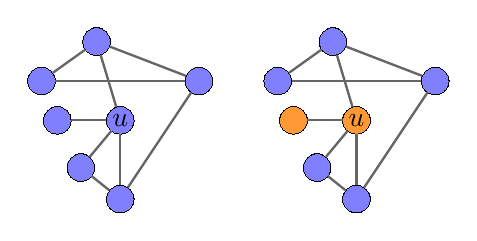
\begin{tikzpicture}[scale=1, auto,swap]

				\node[major] (v_1) at (-2, 0) {$u$};
				\node[major] (v_2) at (-2.3, 1) {};
				\node[major] (v_3) at (-2, -1) {};
				\node[major] (v_4) at (-2.8, 0) {};
				\node[major] (v_5) at (-3, .5) {};
				\node[major] (v_6) at (-2.5, -.6) {};
				\node[major] (v_7) at (-1, .5) {};

				\draw[edge] (v_1) -- (v_2);
				% \draw[edge] (v_3) -- (v_2);
				\draw[edge] (v_1) -- (v_4);
				\draw[edge] (v_7) -- (v_2);
				\draw[edge] (v_5) -- (v_7);
				\draw[edge] (v_3) -- (v_6);
				% \draw[edge] (v_3) -- (v_2);
				\draw[edge] (v_3) -- (v_1);
				% \draw[edge] (v_6) -- (v_7);
				\draw[edge] (v_1) -- (v_6);
				\draw[edge] (v_7) -- (v_3);
				\draw[edge] (v_2) -- (v_5);

				\node[minor] (u_1) at (1, 0) {$u$};
				\node[major] (u_2) at (.7, 1) {};
				\node[major] (u_3) at (1, -1) {};
				\node[minor] (u_4) at (.2, 0) {};
				\node[major] (u_5) at (0, .5) {};
				\node[major] (u_6) at (.5, -.6) {};
				\node[major] (u_7) at (2, .5) {};

				\draw[edge] (u_1) -- (u_2);
				% \draw[edge] (u_3) -- (u_2);
				\draw[edge] (u_1) -- (u_4);
				\draw[edge] (u_7) -- (u_2);
				\draw[edge] (u_5) -- (u_7);
				\draw[edge] (u_3) -- (u_6);
				% \draw[edge] (u_3) -- (u_2);
				\draw[edge] (u_3) -- (u_1);
				% \draw[edge] (u_6) -- (u_7);
				\draw[edge] (u_1) -- (u_6);
				\draw[edge] (u_7) -- (u_3);
				\draw[edge] (u_2) -- (u_5);
			\end{tikzpicture}
			\caption{Emergence of a local minority. 
			On the leftthand side, a sample component from a fully-fragmented network, in which all nodes have opinion $0$ (blue). 
			On the right, the same component after a mutation and voting step, generating two opinion $1$ (orange) nodes.} \label{fig:majorities}
		\end{figure}

		The importance of the local majority/minority distinction is that voting events by the two types of nodes have qualitatively different impacts on the edge density vector $\x$. 
		It is useful to name these two types of events. 
		In \emph{forward} votes, a member of the local majority adopts the opinion of the local minority, spreading the initial mutation. 
		In \emph{backward} votes, a member of the local minority adopts the opinion of the local minority, causing the initial mutation to retreat.  
		We emphasize that these two classes of events are distinct from the label-based classes $0\mapsto 1$ and $1 \mapsto 0$ events in that the label-based classes occur with equal frequency and at equilibrium have symmetric (equal and opposite) expected impacts on $\X$.
		In contrast, forward votes are more frequent and tend to increase $\rho$ by more than backward votes decrease it.  
		To see why, consider the sample scenario shown in \cref{fig:breaking_illustration}. 
		Opinion $1$ (orange) is a local minority in a component statistically dominated by opinion $0$ nodes (blue). 
		We join the action (\cref{subfig:first}) just after a forward voting event has resulted in node $u$ changing its opinion $0 \mapsto 1$. 
		We restrict attention to the three active edges attached to $u$, and start a local clock $\tau_u \in \mathbb{Z}_+$ that counts the number of events that remove a discordant edge from $u$ \pjm{This local clock confuses me and I'm not sure it really buys us that much here in this paragraph? Does anything bad happen if we simply remove it from the discussion?}\pc{I do think we need a way to note that we are only counting events ``near'' $u$. Do you think that just saying that in words would be clearer?}. 
		At time $\tau_u = 0$, voting events along $u$'s active edges are symmetrical: the probability of forward and backward votes are equal. 
		A forward vote adds $2$ net active edges, while a backward vote removes $2$ net active edges. 
		This symmetry is broken by subsequent rewiring and voting events.
		\Cref{subfig:second} shows one possible realization at local time $\tau_u = 2$, in which two active edges have been rewired away from $u$. 
		While a forward vote still adds $2$ net active edges, a backward vote now has no net impact on the active edge density. 
		Intermediate voting events have even greater impact on the behavior of backward voting. 
		In \cref{subfig:third}, two forward voting events have taken place on active edges attached to $u$. 
		A backward vote by $u$ at this moment would remove $2$ net active edges. 
		These phenomena may be observed in simulation data, shown in \Cref{sec:simulation_symmetry} \pjm{Are you still planning to add this figure?}. \pc{Currently it's in the supplementary, and the crossref isn't rendering on Overleaf. Opinion on whether it should be main text?}
		
		\begin{figure}
			\centering
			\begin{subfigure}{.3\textwidth}
				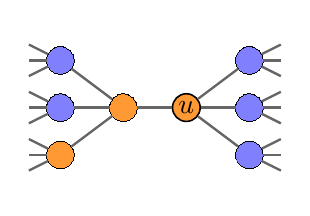
\begin{tikzpicture}[scale=.8, auto,swap]

					\node[focus] (u) at (0,0) {$u$};
					\node[minor] (u_1) at (-1,0) {};
					% \node[minor] (u_2) at (-2,0) {};
					\node[minor] (u_2) at (-2, -.75) {};
					\node[major] (v_4) at (-2, 0) {};
					\node[major] (v_5) at (-2, .75) {};
					
					\draw[edge] (u_1) -- (u_2);
					\draw[edge] (u_1) -- (v_4);
					\draw[edge] (u_1) -- (v_5);

					\foreach \source in {u_2, v_4, v_5}{
						\draw[edge] (\source) --++ (-.5, .25);
						\draw[edge] (\source) --++ (-.5, 0);
						\draw[edge] (\source) --++ (-.5, -.25);
					}


					\draw[edge] (u) -- (u_1);
					% \draw[conc] (u_1) -- (u_2);

					\node[major] (v_1) at (1, .75) {};
					\node[major] (v_2) at (1, 0) {};
					\node[major] (v_3) at (1, -.75) {};

					\draw[edge] (u) -- (v_1);
					\draw[edge] (u) -- (v_2);
					\draw[edge] (u) -- (v_3);

					\draw[edge, white] (v_1) --++ (-1, .5);
					\draw[edge, white] (v_3) --++ (-1, -.5);

					\foreach \source in {v_1, v_2, v_3}{
						\draw[edge] (\source) --++ (.5, .25);
						\draw[edge] (\source) --++ (.5, 0);
						\draw[edge] (\source) --++ (.5, -.25);
					}
				\end{tikzpicture}
				\caption{$\tau_u = 0$}\label{subfig:first}
			\end{subfigure}
			\begin{subfigure}{.3\textwidth}
				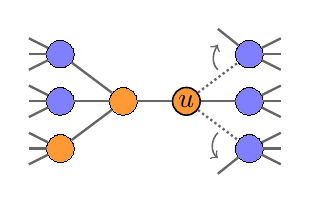
\begin{tikzpicture}[scale=.8, auto,swap]

					\node[focus] (u) at (0,0) {$u$};
					\node[minor] (u_1) at (-1,0) {};
					% \node[minor] (u_2) at (-2,0) {};
					\node[minor] (u_2) at (-2, -.75) {};
					\node[major] (v_4) at (-2, 0) {};
					\node[major] (v_5) at (-2, .75) {};
					
					\draw[edge] (u_1) -- (u_2);
					\draw[edge] (u_1) -- (v_4);
					\draw[edge] (u_1) -- (v_5);

					\foreach \source in {u_2, v_4, v_5}{
						\draw[edge] (\source) --++ (-.5, .25);
						\draw[edge] (\source) --++ (-.5, 0);
						\draw[edge] (\source) --++ (-.5, -.25);
					}

					\draw[edge] (u) -- (u_1);
					% \draw[conc] (u_1) -- (u_2);

					\node[major] (v_1) at (1, .75) {};
					\node[major] (v_2) at (1, 0) {};
					\node[major] (v_3) at (1, -.75) {};

					% \draw[edge] (u) -- (v_1);
					\draw[edge] (u) -- (v_2);
					% \draw[edge] (u) -- (v_3);

					\foreach \source in {v_1, v_2, v_3}{
						\draw[edge] (\source) --++ (.5, .25);
						\draw[edge] (\source) --++ (.5, 0);
						\draw[edge] (\source) --++ (.5, -.25);
					}

					\draw[edge] (v_1) --++ (-.5, .4);
					\draw[edge] (v_3) --++ (-.5, -.4);

					\draw[gone] (u) -- (v_1);
					\draw[gone] (u) -- (v_3);

					\draw[arrow] (.5,.5) [out=135, in=240] to (.5, .9);
					\draw[arrow] (.5,-.5) [out=225, in=140] to (.5, -.9);
				\end{tikzpicture}
				\caption{$\tau_u = 2$}\label{subfig:second}
			\end{subfigure}
			\begin{subfigure}{.3\textwidth}
				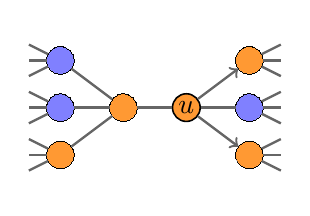
\begin{tikzpicture}[scale=.8, auto,swap]

					\node[focus] (u) at (0,0) {$u$};
					\node[minor] (u_1) at (-1,0) {};
					% \node[minor] (u_2) at (-2,0) {};
					\node[minor] (u_2) at (-2, -.75) {};
					\node[major] (v_4) at (-2, 0) {};
					\node[major] (v_5) at (-2, .75) {};
					
					\draw[edge] (u_1) -- (u_2);
					\draw[edge] (u_1) -- (v_4);
					\draw[edge] (u_1) -- (v_5);

					\foreach \source in {u_2, v_4, v_5}{
						\draw[edge] (\source) --++ (-.5, .25);
						\draw[edge] (\source) --++ (-.5, 0);
						\draw[edge] (\source) --++ (-.5, -.25);
					}

					\draw[edge] (u) -- (u_1);
					% \draw[conc] (u_1) -- (u_2);

					\node[minor] (v_1) at (1, .75) {};
					\node[major] (v_2) at (1, 0) {};
					\node[minor] (v_3) at (1, -.75) {};

					% \draw[edge] (u) -- (v_1);
					% \draw[edge] (u) -- (v_2);
					% \draw[edge] (u) -- (v_3);

					\foreach \source in {v_1, v_2, v_3}{
						\draw[edge] (\source) --++ (.5, .25);
						\draw[edge] (\source) --++ (.5, 0);
						\draw[edge] (\source) --++ (.5, -.25);
					}

					% \draw[edge] (v_1) --++ (-.5, .4);
					% \draw[edge] (v_3) --++ (-.5, -.4);

					\draw[edge, ->] (u) -- (v_1);
					\draw[edge, ->] (u) -- (v_3);
					\draw[edge] (u) -- (v_2);

					\draw[edge, white] (v_1) --++ (-1, .5);
					\draw[edge, white] (v_3) --++ (-1, -.5);
					% \draw[edge] (v_2) -- (v_3);

					% \draw[arrow] (.6,-.05) [out=-90, in=180] to (.95, -.3);
					% \draw[arrow] (.5,.5) [out=135, in=240] to (.5, .9);
					% \draw[arrow] (.5,-.5) [out=225, in=140] to (.5, -.9);
				\end{tikzpicture}
				\caption{$\tau_u = 2$}\label{subfig:third}
			\end{subfigure}
			\caption{
				Schematic illustration of symmetry breaking.
				In \cref{subfig:first},  node $u$ has just changed opinion from $0$ (blue) to $1$ (orange). 
				We start a local clock $\tau_u \in \mathbb{Z}_+$ that counts the number of events that remove a discordant edge from $u$. 
				At this moment, a backwards voting event by $u$ removes a net of 2 active edges.  
				\Cref{subfig:second} shows a sample evolution of the state of $u$ at local time $\tau_u = 2$ after two rewiring events. 
				A backwards voting event by $u$ has no net impact on the active edge density. 
				\Cref{subfig:third} illustrates an alternative scenario at $\tau_u = 2$, in which two forward votes have taken place along active edges attached to $u$. 
				}\label{fig:breaking_illustration}
		\end{figure}

\section{Analytical Methods} \label{sec:analytic}
	We now develop an analytical framework that leverages the asymmetry between forward and backward votes to produce accurate approximations for $\rho^*(\q; c, \alpha)$, the equilibrium density of discordant edges given the opinion density $\q$ and parameters $c$ and $\alpha$. 

	Let $\x(t) = \E[\X(t)]$. 
	Conditioning on event types, the dynamics in $\x$ may be written
	\begin{align}
		m(\x(t+1) - \x(t)) = \lambda \mathbf{w}(\mathcal{G}(t)) + (1-\lambda)\alpha \mathbf{r}(\mathcal{G}(t)) + (1-\lambda)(1-\alpha) \mathbf{v}(\mathcal{G}(t))\;, \label{eq:dynamics}
	\end{align}
	where $\mathbf{w}$, $\mathbf{r}$, and $\mathbf{v}$ are functions of the graph state $\mathcal{G}(t)$ giving the increments in $\x$ due to mutation, rewiring, and voting, respectively. 
	Importantly, however, $\mathbf{w}$ and $\mathbf{r}$ depend only on $\q$ and $\x$, the zeroth and first moments of $\mathcal{G}$ \pjm{It's actually the first and second moments of the opinion distribution on $\mathcal{G}$, right?}\pc{Guess it depends on whether the ``$n$th'' moment refers to expectations involving $n$ edges or $n$ nodes. No problem to use the latter convention} . 
	To write out $\mathbf{w}$, it is useful to introduce the notation $\mathbf{c}$ with components $c_{ij} = c\frac{x_{ij}}{q_i}$ denoting the average number of neighbors of type $j$ of a node of type $i$. 
	Note that, while $x_{ij} = x_{ji}$, $c_{ij} \neq c_{ji}$ for $\q \neq \left(\frac{1}{2}, \frac{1}{2}\right)$. 
	We can then write \pjm{Is this an improvement? Why not write it in terms of $\x$, as already indicated here?}
	\begin{align*}
		w_{ij}(\mathcal{G}) = w_{ij}(\x) = 
		\begin{cases}
			\q_{0}(c_{10} - c_{00}) &  i = j = 0 \\ 
			\q_1 (c_{01}-c_{11}) & i = j = 1 \\ 
			\q_0 (c_{00}  - c_{10}) +  \q_1(c_{11}-c_{01}) & i \neq j\;.
		\end{cases}
	\end{align*}
	To compute $\mathbf{r}$, we write \pjm{Easier to understand if you write it in the same form as w was just written?}\pc{I take your point. I don't think I see how that would work in context -- was there a compact and symmetric format that you had in mind?}
	\begin{align*}
		\mathbf{r}(\mathcal{G}) = \mathbf{r}(\q) = 
		\begin{cases}
			\left(\q_0, -\frac{1}{2}, -\frac{1}{2}, \q_1\right) & \text{rewire-to-random}\\
			\left(1, -1, -1, 1\right) & \text{rewire-to-same}.
		\end{cases}
	\end{align*}
	The difficulty arises in that the voting function $\mathbf{v}$ cannot be similarly parsed exactly in any fixed, finite set of system moments \cite{Demirel2012}. 
	We may therefore view the short-timescale dynamics of $\x$ as the superposition of a Markovian process (in the space of $\q$ and $\x$) governed by mutation and rewiring with a non-Markovian process governed by voting. 
	
	\subsection{Phase Transition}
		Our analytical strategy is to replace the non-Markovian term with a Markovian approximation near the phase transition, which we do using the observations about the symmetry-breaking behavior discussed above. 
		We will suppose that 
		\begin{align}
			\mathbf{v}(\mathcal{G}) \approx \hat{\mathbf{v}}(\q, \x)\;, \label{eq:markov}
		\end{align}
		when $\rho \ll \frac{1}{2}$, which is a first-order Markovian assumption on $\x$ as a function of $\q$. 
		In this sense, our approach is similar to the common pair approximation (PA). 
		However, whereas the PA is a general approach that relies on a closure approximation, we here use the broken symmetry between forward and backward votes to directly develop more accurate approximations. 

		We fix node $u$, and suppose, as in \Cref{fig:breaking_illustration}, that at time $\tau = 0$, $u$ changed its opinion from $j \in \{0,1\}$ to $i \in \{1,0\}$ due to either a mutation or a voting step. 
		As a result of this event, $u$ now possesses certain (random) numbers $J_0$ of inactive and $K_0$ of active edges, whose distributions depend on $\q$, $\x$, and possibly higher-order moments as well.
		To approximate $\hat{v}$, we track each of the $K_0$ discordant edges until each of them has been made concordant, logging voting events along the way. 
		By doing so, we are able to distinguish between forward and backward votes, approximating both the frequency and impact of each on $\x$. 
		Averaging over those events thus provides an approximation for $\mathbf{v}$.
		The quality of the approximation depends on the extent to which the relative frequencies and effects of the tracked voting events reflect those which occur in the true system. 

	Assumptions of timescale separation and mean field majorities together make our calculation tractable.
	We assume that the remainder of $\mathcal{G}$ is changing slowly relative to the ego network of node $u$, so that only dynamics that sample the initial $K_0$ edges need to be accounted for. 
			This assumption will be strongest when $\rho \ll 1$ and $\lambda \ll 1$. 
	We also assume that nodes in the local majority have degree distributions governed by the global network average $\x$. 
		The mean-field approximation is used to approximate the distributions of $J_0$ and $K_0$. 
		Under our hypotheses, node $u$ was in the local majority in the immediately previous time-step before we joined the action (when node $u$ became a local minority node).
		This allows us to approximate the distributions of $J_0$ and $K_0$ in terms of $\q$ and $\x$. 
		In particular, we have that $\E[K_0] = c_{00}$. Meanwhile, $\E[J_0] = 1 + c_{01}$ if $u$ emerged as a forward vote or $\E[J_0] = 0$ if $u$ emerged as a mutation. 
		In the approximations below, we model each of $K_0$ and $J_0$ as truncated Poisson random variables with the appropriate averages. 

		We now define notation to track the various types of voting events. 
		Let $R$ be a random variable giving the number of voting events by neighbors of $u$. 
		By the timescale separation assumption, we may assume that each such vote happens along one of the $K_0$ initial active edges. 
		Since $u$ is assumed to be in the local minority, votes by neighbors are forward votes. 
		Let $W$ give the number of voting events by nodes not attached to $u$ due to one of the $K_0$ active edges \pjm{Looking for clarification: can we simply use the phrase you have in the ``rewire-to-random'' sentence to say clearly what this?}. 
		In the case of the rewire-to-same model, no such events occur. 
		In the rewire-to-random model, these events occur when an edge attached to $u$ is rewired in such a way that it is no longer attached to $u$, but to another node of the same opinion. 
		Let $\1_u$ be the indicator variable that $u$ changes its vote (i.e. votes backwards) prior to all $K_0$ active edges being resolved. 

		These variables will count the voting events, but we also require vectors to track the impact of a given event on $\x$. 
		Under the mean-field assumption, forward votes are governed by the global mean degrees $\C$. 
		The expected impact on $\x$ of votes counted by $R$ when $\mathcal{L}_u = 1$ on a component dominated by $0$s is given by \pjm{I'm admittedly a little confused by notation: can we be more explicit about the relationship between $R$ and the $\mathbf{h}$ items?}
		\begin{align}
			\mathbf{h}_1(\C) = \frac{1}{2}\left(-2c_{00} , c_{00} - c_{01} - 1, c_{00} - c_{01} - 1, 2(1+c_{01})\right)^T\;.
		\end{align}
		Interchanging the opinion indices gives the analogous expression for $\mathbf{h}_0$, the impact of forward votes when $u$ has opinion $0$ on a component dominated by $1$s. 
		Votes counted by $W$ are again mean-field approximated. 
		Since these edges are no longer connected to $u$, their impact is independent of $i$. 
		We then have \pjm{I think the notation is a little confusing because we have $\mathbf{w}$ above for mutation events. Should we change the letter here (and, if so, in the previous paragraph---indeed, should we restructure this paragraph and the one above to more clearly separate the two counts (currently $R$ and $W$)?}
		\begin{align}
			\mathbf{w}(\C) = \frac{\mathbf{h}_0(\C) + \mathbf{h}_1(\C)}{2}\;.
		\end{align}

		It remains to consider the impact of a backward vote by $u$, for which the analysis is more subtle. 
		This term has components
		\begin{align}
			\mathbf{b}_1(\q, \C) = \left(2\E[K|1], \E[J-K|1], \E[J-K|1], -2\E[J|1]\right)\;,
		\end{align}
		where $J$ (respectively, $K$) are the number of inactive (active) edges attached to $u$ at the time of voting. 
		The expectations are conditioned on $\mathcal{L}_u = 1$.  
		With these terms, the expected increment in the edge counts due to voting is given by the 4-vector
		\begin{align}
			\hat{\mathbf{v}}(\q, \x) = \frac{1}{2} \sum_{i \in \{0,1\}} \frac{\E[R|i]\mathbf{h}_i(\C) + \E[W|i]\mathbf{w}(\C) + \E[\1_u\mathbf{b}_i(\mathbf{q},\mathbf{c})|i]}{\E[R + S + \1_u|i]}\;. \label{eq:v_hat}
		\end{align}
		To complete the approximation scheme it remains only to compute the various expectations. Under the timescale-separation and mean-field approximations, this is possible analytically, as derived in \Cref{sec:calcs}: \pjm{In light of the short length of the supplement, I'm thinking we might be able to get away with it as an Appendix here instead? That's not a decision we need to make until we're all but ready to submit.}   
		\begin{equation}
			\begin{aligned}
				\E[R|i] &= 1 - \phi_{K_0}(\beta_i) \\ 
				% \E[R|i] &= 1 - \E_{K_0}[\beta_i^{K_0}] \\ 
				% \sum_{j,k} p_{K_0|I}(k|i)\left((1-\beta_i^{k})\left(1 +  \frac{\beta_i\sigma_i (1 + \eta_i)}{1-\beta_i}\right)\right) \\ 
				\E[\1_uK|i] &= \E[K_0|i] - \frac{\beta_i}{1-\beta_i}(1-\phi_{K_0}(\beta_i)) \\ 
				% \E[K|i] &= \E_{K_0}\left[K_0 - \frac{\beta_i(1-\beta_i^{K_0})}{1-\beta_i}\right] = \sum_k p_{K_0|I}(k|i)\left( k  - \frac{\beta_i(1-\beta_i^{k})}{1-\beta_i}\right) \\ 
				\E[\1_uJ|i] &= \E[J_0|i] + \eta_i(\E[K_0|i] - \E[K|i]) \\
				% \E[J|i] &= \sum_{k,j} p_{K,J|I}(k,j|i) (j + \eta_i(k - \E[K|i])) \\ 
				\E[\1_u|i] &= \E[R|i] = 1 - \phi_{K_0}(\beta_i) \\ 
				\E[W|i] &= \sigma_i\E[K_0 + J_0 - \1_u(K - J)|i]\;,	
				% \E[\1_u|i] &= \E_{K_0}[(1-\beta_i^{K_0})] &= \sum_k p_{K_0|i}(k|i)(1-\beta_i^k)
			\end{aligned} \label{eq:component_approx}
		\end{equation}
		where the rates $\beta_i, \sigma_i, \eta_i$ are functions of $\q$, $\alpha$, and $i$, and independent of $\x$; $\phi_{K_0}(z) = \sum_{k = 1}^\infty \prob(K_0 = k) z^{k}$ is the probability generating function of $K_0$; and the various expectations are computed over the joint distribution $p_{J_0, K_0}(\cdot;\C)$ of $J_0$ and $K_0$. 
		  
		
		
		\begin{figure}
			\centering
				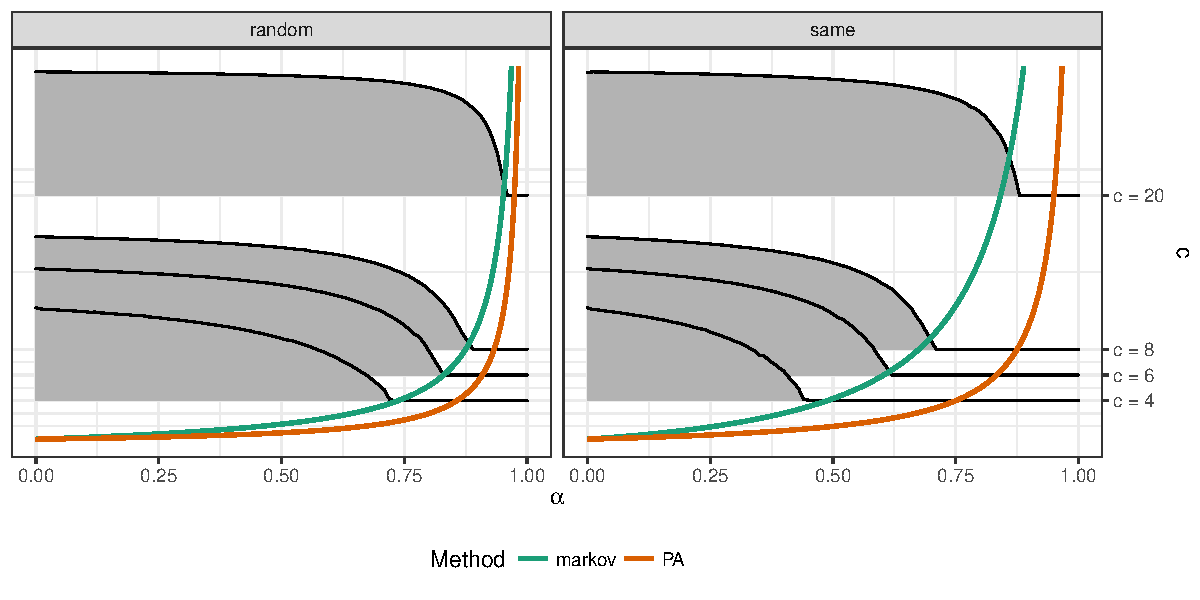
\includegraphics[width=1\textwidth]{transition_joy}
			\caption{Approximating the phase transition. 
			Grey ridges give simulation traces from networks with $n = 10^4$ nodes, $\lambda = 2^{-16}$, and varying $c$ and $\alpha$. 
			The green curve gives the analytic prediction of the phase transition found by numerically solving \Cref{eq:transition_approx} via least-squares. 
			The orange curve gives the pair approximation (PA) as derived in \cite{Durrett2012} for each model variant.}
			\label{fig:transition_joy}
		\end{figure}

		With the expression \Cref{eq:v_hat} in place, we may then approximate the long-term dynamics of $\x$ under \Cref{eq:dynamics}, subject to the constraint that the components of $\x$ sum to unity. 
		We write $\hat{\x}(\q; \alpha)$ for the limit point of the dynamics. \todo{Uniqueness of $\hat{\x}$?}
		The approximation is subcritical when $\hat{\rho}(\q; \alpha) \triangleq 2\hat{\x}_{01}(\q; \alpha) = 0$, and supercritical otherwise. 
		Solving 
		\begin{align}
			\alpha^*(\q) = \max \{\alpha : \hat{\rho}(\q; \alpha) = 0\} \label{eq:transition_approx}
		\end{align}
		gives our approximation for the phase transition. 

		\Cref{fig:transition_joy} shows the approximate phase transitions computed using \Cref{eq:transition_approx} for varying $c$, in green, when $\q = \left(\frac{1}{2}, \frac{1}{2}\right)$. % \footnote{Empirically, the rewire-to-random curve phase transition can also be computed by solving $\phi_{K_0}(\beta_i^{K_0}) \approx \frac{1}{2}$ for $\alpha$, which has a branching-process intuition behind it and leads to a much cleaner calculation. Intriguingly, the right constant for the rewire-to-same case appears to be $\phi_{K_0}(\beta_i^{K_0}) \approx \frac{1}{3}$} 
		Compared to the standard pair approximation (orange), the present approximation approach is substantially more accurate.
		Indeed, the calculation of the transition for the rewire-to-random model is the most accurate we know of, while the calculation for the rewire-to-same model is competitive with existing approaches.
		The approximation of the phase transition is more accurate than the Approximate Master Equations (AMEs) of \cite{Durrett2012} and the partial differential equation approach of \cite{Silk2014}. 
		The fan-motif method used by \cite{Bohme2011} to estimate the rewire-to-same phase transition is somewhat more accurate in that case, but also higher-dimensional, requiring a bisection search in $\alpha$ in which each stage computes the leading eigenvalue of a $(c-1)\times (c-1)$ matrix. 

		As discussed in \cite{Durrett2012} and shown in \Cref{fig:arch_illustration}, the phase transitions in the two models differ in their sensitivity to $\q$. 
		This behavior is reflected algebraically in \Cref{eq:component_approx}.
		As shown in \Cref{sec:SI_phase}, the expressions appearing in \Cref{eq:component_approx} depend on $\q$ in the rewire-to-random model regardless of $\x$. 
		However,  in the rewire-to-same model, dependence on $\q$ emerges only when $\rho > 0$, implying that the phase transition itself is independent of $\q$. 
		Furthermore, the local approximation scheme also gives us a physical interpretation of this mysterious behavior. 
		Consider the emergence of a mutant node $u$ with opinion $1$ on a component of majority opinion $0$. 
		In the rewire-to-random case, the fast local rewiring dynamics depend explicitly on $\q$, the \emph{global} opinion densities. 
		When $\q_1$ is large, an edge attached to $u$ and rewired is more likely to become inactive, resulting in fewer active edges in the neighborhood of $u$. 
		In the rewire-to-same case, however, the fast rewiring does not explicitly depend on $\q$. 
		An active edge attached to $u$ and rewired becomes inactive with probability $1$, regardless of the value of $\q$. 
		The local dynamics are not fully independent of $\q$, but the dependence is mediated by the slow voting dynamics. 
		\todo{This is correct but needs to be made much tighter -- look for a precise punchline.} \pjm{This intuition is really good here. I'm curious, there also seems to be a way in which the model for rewire-to-same has a degenerate behavior at small $\rho$ in that it also implies that one of the opinions is of small population, so then three of the edge types are small. I'm just babbling...}\pc{I'm interested in where you're going here. At the moment, I can't see the distinction between the two models along these lines -- want to elaborate?}
	
	\subsection{Supercritical Equilibria}
		
		We now turn to the approximation of $\rho^*(\q;\alpha)$, the equilibrium density of discordant edges, for $\alpha < \alpha^*$. 
		In this regime, the separation of timescales assumption becomes progressively more inaccurate, and our explicit distinction between forward and backward votes breaks down. 
		In particular, the impact of a single node voting backwards progressively diminishes due to re-randomization of the node's local neighborhood between votes. 
		We address this via simple interpolation to an approximation of the case $\alpha = 0$, which corresponds to a variation of a ``pure'' voter model without rewiring. 
		A simple mean-field argument (given in \Cref{sec:SI_alpha_0}) provides an approximation for the $\alpha = 0$ arch:
		\begin{align}
			\hat{\rho}^*(\q; 0) \approx 2q_1q_2\frac{c-1}{c}\;. \label{eq:alpha_0}
		\end{align}
		We note in passing that, despite the crudeness of this mean-field approximmation, this estimate for the $\alpha = 0$ arch is substantially more accurate than both the pair approximation in \cite{Durrett2012} and the even more sophisticated active-motif approach of \cite{Demirel2012}. 

		We introduce an interpolation function 
		\begin{align}
			s(\x) = \frac{\hat{\rho}^*(\q;0) - \rho}{\hat{\rho}^*(\q;0)}\;, \label{eq:interpolation}
		\end{align}
		to quantify the distance of the system state from the estimated $\alpha = 0$ arch, and then use this interpolation function to introduce decay in the backward voting term of  \Cref{eq:component_approx}.\footnote{While any monotonic transformation of  \Cref{eq:interpolation} may be well-motivated, in practice we found similar numerical results under a variety of such transformations.}
		We then replace $\E[J - K|i]$ with $\E[J - K|i]s(\x)$ to reflect the diminishing influence of backward votes, obtaining 
		\begin{equation}
			\hat{v}(\q, \x) = \frac{1}{2} \sum_{i \in \{0,1\}} \frac{\E[R|i]h_i(\C) + \E[W|i]w(\C) + \E[\1_u(J-K)|i]s(\x)}{\E[R + S + \1_u|i]}\;.  \label{eq:component_approx_super}
		\end{equation}
		\Cref{eq:component_approx_super} may then be substituted back into \Cref{eq:dynamics}; the corresponding solution for $\x$ then yields an approximation of $\mathbf{\rho}$. 
		\begin{figure}
			\centering
				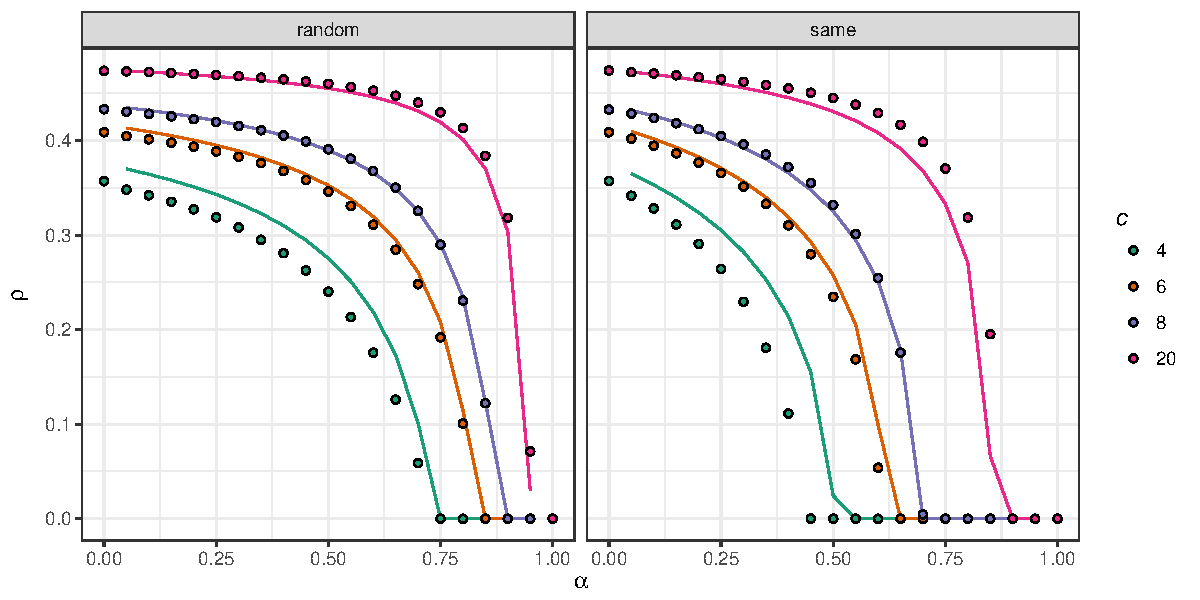
\includegraphics[width=.8\textwidth]{arch_tops}
			\caption{Supercritical equilibria for $\q = \left(\frac{1}{2}, \frac{1}{2}\right)$.
			Dots give simulation traces from a network of $n = 10^4$, $\lambda = 2^{-12}$, and varying $\alpha$ and $c$.
			Solid lines give the approximation to $\rho$ computed by numerically solving \Cref{eq:dynamics} and \Cref{eq:component_approx_super}.} \label{fig:arch_tops}
		\end{figure}
		
		To evaluate the supercritical approximation, we first consider its performance on the standard estimation task with symmetric opinion densities. 
		\Cref{fig:arch_tops} shows the estimate for $\rho$ when $\q = \left(\frac{1}{2}, \frac{1}{2}\right)$ for varying $\alpha$. 
		The rewire-to-random approximations are highly accurate, largely due to the accurate estimate of the phase transition. 
		The approximation deviates from simulations by no more than $5\%$. 
		This overall level of accuracy is comparable with that of the  Approximate Master Equation (AME) approach employed in \cite{Durrett2012}. \pjm{Is it really? Isn't it actually better than the AME result in the Durrett et al. paper? Or are you just being conservative? (Not that there's anything wrong with that!)}\pc{Checking Fig. 10 of \cite{Durrett2012}, it looks like the largest deviation from the data occurs with $\alpha = 0.7$, with a discrepancy $\hat{\rho} - \rho \approx 0.07$ or so, when $c = 4$. The largest deviation for $c = 4$ in our model is around $\alpha = 0.6$ or so, and is maybe $\hat{\rho} - \rho \approx 0.05$ -- better, not wildly. Of course we have advantages -- better near the phase transition, and we can compute for larger $c$. But if you made a version of this plot with AMEs, at least for $c = 4$, it would look a bit better than I think you think it would. =)}
		Interestingly, the two methods are most accurate in dramatically different regimes---whereas the AMEs are nearly exact for small $\alpha$ and decay in quality near $\alpha^*$, our present method is much more accurate near $\alpha^*$ but degrades slightly as $\alpha$ becomes small. 
		In the rewire-to-same case, the approximation is predictably weaker due to the larger error in the estimation of the phase transition. 
		There is larger deviation, on the order of $10\%$, in many of the simulation traces depending on $c$. 
		The overall approximation quality is again comparable to that of AMEs, but is outperformed by certain specialized methods such as the active-motif approach of \cite{Demirel2012}. 
		
		In addition to demonstrating favorable accuracy, the present approximation approach is much lower-dimensional than its competitors. 
		AMEs require the solution of $\Theta\left(k_\mathrm{max}^2\right)$ coupled differential equations; in the $c = \langle k\rangle = 4$ case, the authors of \cite{Durrett2012} used $225$ such equations. 
		This makes the computation of equilibrium approximations computationally prohibitive for even moderate $c$. 
		Active-motif methods also have similar scaling properties. \todo{What actually IS the difference between active-motif methods and AMEs?}
		In contrast, the present method displays constant scaling: there are four nonlinear equations to solve, regardless of the value of $c$. 
		The low-dimensional nature of the approximation also supports useful physical intuition -- each term is meaningful and corresponds to a distinctive event-type when viewed from the local perspective. 
		
		Turning now to the case $\q \neq \left(\frac{1}{2}, \frac{1}{2}\right)$, \Cref{fig:arches} compares the curves obtained by numerically solving \Cref{eq:dynamics} as $\q$ varies. 
		Due to the accurate estimation of the location of the phase transition in $\alpha$, the arches for the rewire-to-random model agree well with the data both on the equilibrium active edge density and on the support of the arch -- the values of $\q$ for which $\rho^*(\q;\alpha) > 0$. 
		Compared to AMEs, the computed arches for the $c = 4$ rewire-to-random case are comparable in overall accuracy, better estimate the correct support, and also better capture the qualitative parabolic shape.  
		The accuracy of the approximation increases with $c$, but comparison to AMEs and active-motif approaches are no longer possible due to the computational costs of the latter two methods. 
		As with the $\q = \left(\frac{1}{2}, \frac{1}{2}\right)$ case, the rewire-to-same results less accurate. 
		The computed arches do correctly span the entire interval $[0,1]$ for the rewire-to-same case (cf.\ the behavior of the rewire-to-random case). 
		The overall numerical accuracy in the $c = 4$ case is comparable to AMEs, but the qualitative parabolic shape has been lost. 
		The reason for this difference is not clear to the authors, and further investigation into this phenomenon is called for. 

		\begin{figure}
			\centering
				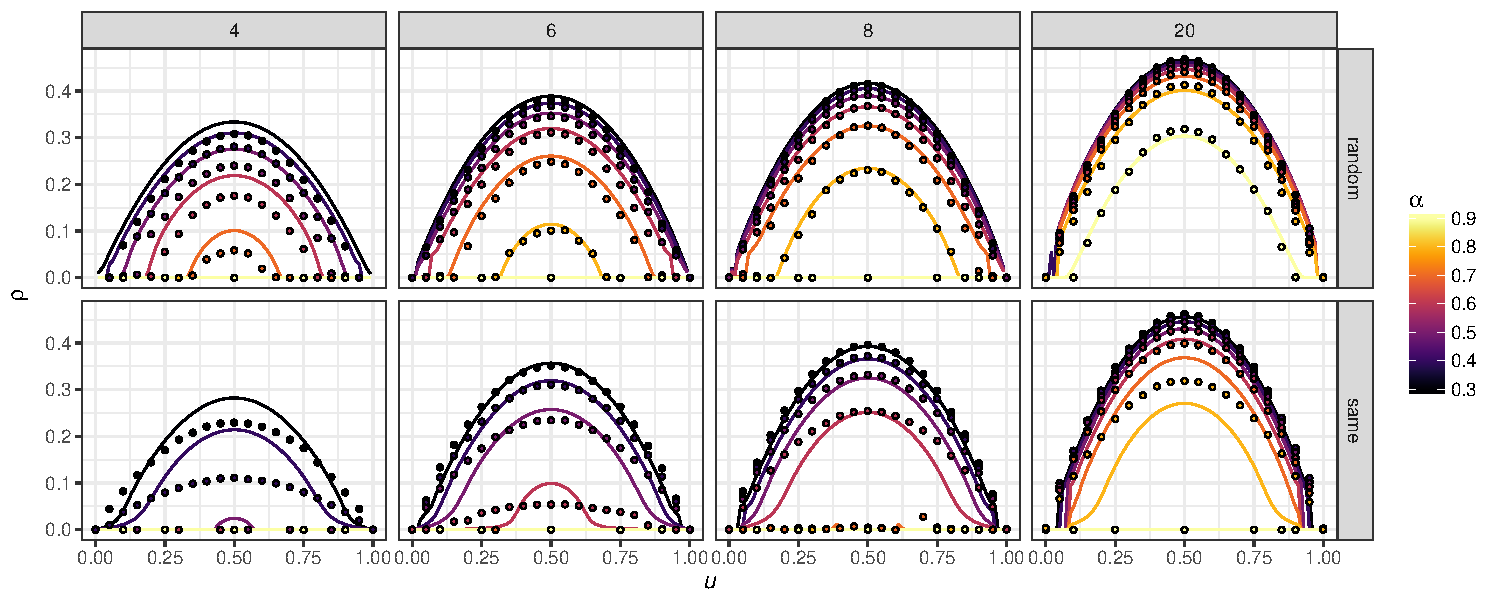
\includegraphics[width=1\textwidth]{arches}
			\caption{Approximations to arches for rewire-to-random and rewire-to-same systems with varying mean degree $c$ and rewiring rate $\alpha$. 
			Curves give theoretical predictions obtained by numerically solving \Cref{eq:dynamics} and \Cref{eq:component_approx_super}. 
			Points give simulation averages traces from networks with $n = 10^4$ nodes,  $\lambda = 2^{-16}$, and varying $\alpha$.}
			\label{fig:arches}
		\end{figure}

\section{Discussion} \label{sec:discussion}

	Adaptive voter models offer a simple rule set generating complex behaviors for how individual decisions about beliefs and social attachments can generate global, opinion-based polarization. 
	While the underlying rules are simple to state, the coevolving nature of the dynamics render these systems very challenging to analyze. 
	We have considered an ergodic adaptive voter model variant which enables a local perspective on fragmentation transitions and other model properties. 
	The local perspective allows us to use the asymmetry of voting events to develop Markovian approximations based on the fast time-scale dynamics around single nodes. 
	The resulting approach is conceptually intuitive, computationally tractable, and empirically accurate. 
	
	One of the most puzzling issues raised by our results is the difference between the accuracies of our approach for the rewire-to-random and rewire-to-same adaptive voter models. 
	While we succeed in characterizing the rewire-to-random arch nearly exactly, the same methods produce poorer results for the rewire-to-same model. 
	We conjecture that the rapid local sorting produced in rewire-to-same dynamics badly violates our mean-field assumption on forward votes, as suggested by the bottom-left panel of \Cref{fig:symmetry_breaking}. 
	It would be interesting to extend our methodology to see whether refinements are possible that better characterize the rewire-to-same behavior, and potentially shed light on the essential features governing the dramatic difference in the nature of the phase transitions in these two models. 
		
	It is also of substantial interest to consider extensions and generalizations. 
	The most natural extension is to the case of multiple opinion states and structured opinion spaces. 
	Previous work on multi-opinion models has been restricted to either characterization of the various phase transitions (\cite{Bohme2012}) or empirical discussion of supercritical equilibrium behavior (\cite{Shi2013}). 
	One explanation for this limitation in scope is computational, in that the number of operations required to compute approximations under active motif and AME approaches are exponential in the number $\abs{\mathcal{X}}$ of opinion states, rendering both methods infeasible. 
	In contrast, likely extensions of our moment-closure methods scale as $\Theta(\abs{\mathcal{X}}^2)$, which would likely be computationally tractable. 
	If accuracy were preserved, such extensions would present the first scalable analytic methods for multi-opinion models. 
	%Further generalizations may also be possible. 
	While we developed our approximations for the specific case of the binary-state AVM, that development relies only on three base ingredients: symmetry-breaking, timescale separation, and mean-field majorities. 
	We conjecture that these ingredients should be present in any adaptive model with homophilic dynamics in which rewiring steps involve uniform selection from an extensive subset of the graph, such as a subset sharing a given node state. 
	An example of a more complex system in which these ingredients are present is the networked evolutionary prisoner's dilemma game of \cite{Lee2017a}, in which nodes display richer strategic behavior in their opinion update and rewiring behavior. 
	Despite this behavior, the existence of a phase transition driven by homophily may allow for the deployment of the Markovian assumption in this case as well. 
	% An example coevolutionary model to which our methods may not be applicable is the transitivity-reinforced dynamics of \cite{Malik2016}. 
	% Because nodes tend to rewire within their neighborhoods, timescale separation may not be a practical assumption. 

	
\section*{Acknowledgments} 
	We are grateful to Feng (Bill) Shi for contributing code used for simulations, and to Patrick Jaillet for helpful discussions. PSC was supported by NSF Graduate Research Fellowship under Grant Number 1122374. PJM was supported by the Eunice Kennedy Shriver National Institute of Child Health \& Human Development of the National Institutes of Health under Award Number R01HD075712. The content is solely the responsibility of the authors and does not necessarily represent the official views of the National Science Foundation or National Institutes of Health.\pc{Amused by the thought that our views here could get NIH in trouble if we didn't have that disclaimer.}

% TODO
%%% Reverse-outline, with special emphasis on introduction, discussion, conclusion.
%%% Revise appropriately
%%% Standardize notation, and consolidate SI
%%% Check figures

\bibliographystyle{siamplain}
\bibliography{refs.bib}{}


\end{document}